\documentclass[12pt]{article}
\usepackage[margin=1in]{geometry}
\usepackage{amsmath,amssymb}
\usepackage{graphicx}
\usepackage{booktabs}
\usepackage[numbers,sort&compress]{natbib}
\usepackage{hyperref}

\title{Target Health Factor based Soft Liquidation with Collateral Restoration for DeFi Lending}
\author{Jianming Liu\\
DefinanceX Capital}
\date{}

\begin{document}

\maketitle

\begin{abstract}
This paper develops a state-contingent partial-liquidation mechanism for collateralized lending in which execution is triggered by LLTV/LTV conditions and liquidation size is computed from target-HF repair requirements. We formalize the mechanism, derive event-level accounting identities, and evaluate behavior in a reproducible multi-loan simulation framework with trigger-level execution logs. We compare fixed-close-factor liquidation, target-HF partial liquidation without buyback, and target-HF buyback under lot-matched, positive-spread, reborrow-funded execution. Across stress-batch and historical-window evidence, target-HF shows a directional advantage signal over fixed-CF but not universal dominance, while buyback provides a statistically robust incremental improvement over no-buyback. Under strict bad-debt feasibility gates, borrower-loss-optimal candidates can disappear in the explored parameter region. The contribution is therefore an auditable mechanism and evaluation protocol that make liquidation-restoration-risk trade-offs explicit, rather than a claim of universal policy dominance.
\end{abstract}

\section{Introduction}
Liquidation is central to solvency in overcollateralized lending. Most deployed systems are built around one or a small number of hard CR thresholds, where falling below the threshold triggers immediate liquidation pressure. In highly volatile markets, this can create cliff effects: borrowers experience abrupt collateral loss, while protocols face concentrated execution risk.

This paper proposes \emph{state-contingent two-sided partial liquidation}, a rule-based alternative that replaces fixed-quantity bucket rules with state-driven actions. As collateral value declines, liquidation is triggered by LTV/LLTV breaches and sized by a dynamic close factor; when risk normalizes, buyback is funded through constrained reborrowing. The objective is not to eliminate liquidation, but to transform it from a discontinuous event into a staged control policy with auditable behavior.

Hard-threshold lending liquidations are widely documented in production protocols such as Aave, where positions are monitored by health-factor style constraints and liquidators repay debt for discounted collateral claims \cite{aave-liquidations}. Target-HF partial-liquidation sizing---where debt repayment is computed to restore the borrower's health factor to a governance-set target rather than applying a fixed close factor---has been formally adopted in Aave v4's liquidation engine \cite{aave-v4-liquidations} and is under active exploration in Morpho-style designs. However, these implementations generally stop at sell-side deleveraging and do not include an endogenous protocol buyback leg for collateral restoration. In contrast, Curve's crvUSD design introduces soft-liquidation ranges through LLAMMA, where collateral is gradually converted across price bands rather than liquidated in one step \cite{curve-crvusd,curve-llamma}.

This paper takes target-HF sizing as a shared starting point and contributes the \emph{buyback restoration} dimension: a lot-matched, positive-spread, reborrow-funded mechanism that allows partial recovery of previously liquidated collateral when market conditions improve. Specifically, the study contributes in three dimensions: (i) a formal LLTV/LTV-based partial-liquidation rule with target-HF repair sizing and explicit sell/recovery triggers; (ii) a transparent accounting decomposition of debt reduction, reserve accumulation, and collateral restoration for pathwise stress diagnostics; and (iii) a reproducible event-level simulation pipeline that supports paired policy comparison under identical paths.

\section{Model Setup}
Consider a loan with debt $D$ (USD), collateral amount $C$ in a generic risky asset, initial asset price $P_0$, and initial collateral ratio $\mathrm{CR}_0>1$.
Initial collateral amount is
\[
C_0 = \frac{D\,\mathrm{CR}_0}{P_0}.
\]

Let LLTV denote the liquidation LTV threshold. For a single-collateral position with debt $D_t$ and collateral value $C_tP_t$, define
\[
\mathrm{LTV}_t = \frac{D_t}{C_tP_t}, \qquad
\mathrm{HF}_t = \frac{C_tP_t\,\mathrm{LT}}{D_t}=\frac{\mathrm{LT}}{\mathrm{LTV}_t}.
\]
Liquidation eligibility is state-defined: a sell action is considered when $\mathrm{LTV}_t\ge \mathrm{LLTV}$ (equivalently when HF enters the liquidation region implied by LT/LLTV calibration).

\paragraph{Endogenous partial liquidation via LLTV/LTV.}
In the current implementation, partial liquidation is sized to restore the position toward a target health factor $\mathrm{HF}^{\star}$, rather than using a fixed liquidation amount. When $\mathrm{LTV}_t\ge \mathrm{LLTV}$, the engine computes the debt reduction required to move the post-trade state to the target region. With liquidation bonus $b\ge0$, sell quantity is
\[
q_t^{\text{sell}}=\frac{(1+b)\Delta D_t}{P_t},
\]
and the target-HF condition is
\[
\mathrm{HF}^{\star}=\frac{\left(C_t-\frac{(1+b)\Delta D_t}{P_t}\right)P_t\,\mathrm{LT}}{D_t-\Delta D_t}.
\]
Solving gives the target repayment proposal
\[
\Delta D_t^{\star}=\frac{\mathrm{HF}^{\star}D_t-\mathrm{LT}\,C_tP_t}{\mathrm{HF}^{\star}-\mathrm{LT}(1+b)},
\]
which is then clipped by debt and available collateral constraints.

If price continues to fall after the first repair trade, the position can re-enter the liquidation region and trigger a second partial liquidation. The pair $(P_{t_1},P_{t_2})$ together with executed quantities $(q_{t_1}^{\text{sell}},q_{t_2}^{\text{sell}})$ defines an empirical liquidation price band and quantity profile, which serves as the state-derived basis for subsequent two-sided execution. In the implemented simulator, buyback is lot-matched: each recovery buy is matched to an open previously sold lot (partial matching allowed), and execution is allowed only when the expected grid spread is positive.

Buyback is enabled under a risk-guard condition, implemented as
\[
\mathrm{LTV}_t\le \mathrm{LLTV}+\delta,
\]
where $\delta\ge0$ is a buyback risk-guard bandwidth. For an open sell lot $i$ with quantity $q_i^{\text{sell}}$ and sell price $P_i^{\text{sell}}$, buyback executes only if
\[
P_t < P_i^{\text{sell}}\quad\text{and}\quad q_i^{\text{sell}}P_t \le B_t,
\]
and then the executed buyback quantity is lot-constrained:
\[
0 < q_t^{\text{buy}} \le q_i^{\text{sell}}.
\]
The aggregate target remains capped by buyback ratio $\eta\in(0,1]$ via $Q_t^{\text{bought,total}}\le\eta Q_t^{\text{sold,total}}$.

Relative to a stricter guard $\mathrm{LTV}_t\le\mathrm{LLTV}-\delta$, using $\mathrm{LLTV}+\delta$ is intended to activate restoration earlier during rebounds and to reduce missed recovery opportunities in choppy regimes. This choice introduces an overlap interval $[\mathrm{LLTV},\mathrm{LLTV}+\delta]$ where sell and buy conditions can both hold in principle. In implementation, conflict is resolved deterministically by execution order: sell logic is evaluated first, and buyback is checked only on the post-sell state within the same step.

\section{Mechanism and Accounting}
The mechanism maintains an execution state and inventory record per position. A sell event is triggered by an LLTV breach ($\mathrm{LTV}_t\ge\mathrm{LLTV}$); its size is computed online from the target-HF repair requirement, debt, and price. A buy event is governed by a risk guard ($\mathrm{LTV}_t\le\mathrm{LLTV}+\delta$), and executes only if it strictly matches an open sell lot under positive expected grid spread and reborrow-capacity constraints. In terminal states, the policy may allow loss-making buyback during sufficiently strong recovery; this preserves explicit restoration semantics rather than purely myopic profit maximization.

Operationally, each sell event includes a liquidation bonus buffer. Let gross sell proceeds be $q_t^{\text{sell}}P_t$ and debt reduction be $\Delta D_t$; then reserve increment is $\Delta U_t=q_t^{\text{sell}}P_t-\Delta D_t$. This buffer is the first-loss-absorbing source for subsequent buyback operations and can be interpreted as the economic budget that funds recovery commitments. Consequently, occasional terminal buyback losses are not treated as model failure, but as bounded drawdowns against cumulative liquidation-buffer income.

Because the mechanism has both downward (sell) and upward (buyback) actions, execution can be permissionless on both sides. In practice, this implies two directions of keeper/liquidator participation: one side competes to execute debt-reducing sell liquidations, while the other side competes to execute inventory-restoring buybacks when recovery triggers are met. This two-sided design reduces reliance on a privileged actor and improves liveness under volatile conditions.

Protocol USD inventory evolves from sell and buy events, and borrower collateral inventory evolves inversely. Collateral value at time $t$ is
\[
V_t = C_t P_t + U_t,
\]
where $C_t$ is borrower collateral amount and $U_t$ is protocol-held USD from prior sells. The realized CR is $\mathrm{CR}_t = V_t / D$.

\paragraph{Risk trade-offs and interpretation.}
Event-level realized protocol P\&L is
\[
\Pi_k = q_k(P_k^{\text{sell}} - P_k^{\text{buy}}),
\]
and total P\&L is $\Pi=\sum_k \Pi_k$ over completed sell-buy cycles (including terminal recovery if executed).

To make tail effects explicit, we decompose total outcome as
\[
\Pi_{\text{total}} = \sum_{k\in \mathcal{K}_{\text{normal}}} \Pi_k + \Pi_{\text{terminal buyback}},
\]
where the first term is typically positive under repeated two-sided execution, while the terminal term can be negative in adverse rebound paths.

Accordingly, the mechanism should be interpreted as conditionally profitable rather than deterministically profitable: for a given parameterization and market path, expected net P\&L can be positive, but positive profit is not guaranteed in every realization.

Two properties are central:

\noindent\textbf{Path dependence} is fundamental: identical terminal prices can generate materially different outcomes if crossing order and dwell time differ. \textbf{Restoration--releverage trade-off} is equally central: larger recovery-side buybacks improve borrower-side restoration but require debt re-expansion within borrowing-capacity limits.

This mechanism therefore reallocates liquidation risk over time instead of concentrating it at a single boundary.

\section{Simulation Framework and Experimental Results}
This section reports a unified evaluation pipeline for the implemented mechanism. The objective is mechanism validation under path uncertainty: we evaluate borrower outcomes, solvency/tail risk, and execution behavior under both synthetic stress batches and rolling historical windows.

\subsection{Experimental design and policy set}
All experiments compare three policies under matched initial conditions and matched price paths:
\begin{itemize}
  \item \texttt{traditional\_fixed\_cf}: fixed close-factor liquidation without buyback,
  \item \texttt{target\_hf\_no\_buyback}: target-HF partial liquidation with buyback disabled,
  \item proposed target-HF with buyback (scenario key \texttt{baseline\_dynamic}): target-HF partial liquidation with strict buyback.
\end{itemize}
For the dynamic policy, buyback is constrained to lot-matched, positive-spread, reborrow-funded execution. Specifically, each buy must match an open sell lot, execute only when buy price is below the matched sell price, and satisfy borrowing-capacity constraints. This keeps restoration behavior auditable and avoids reserve-funded shortcuts.

\subsection{State variables, metrics, and implementation alignment}
At each step, the simulator records
\[
\mathrm{HF}_t = \frac{C_tP_t\,\mathrm{LT}}{D_t},\qquad
\mathrm{LTV}_t = \frac{D_t}{C_tP_t},\qquad
\mathrm{CR}_t = \frac{C_tP_t}{D_t}.
\]
Sell triggers are evaluated at $\mathrm{LTV}_t\ge\mathrm{LLTV}$ and buyback guard at $\mathrm{LTV}_t\le\mathrm{LLTV}+\delta$. Event logs include debt repayment, collateral sold/bought, reserve changes, and trigger-level snapshots.

Primary evaluation metrics are borrower final loss, restoration ratio $\rho=C_T/C_0$, peak bad debt $\max_t\max(0,D_t-C_tP_t)$, event turnover (sell/buy intensity), and minimum health factor. We report both central tendency and tail-sensitive statistics to avoid selecting policies that only win in average-case regimes.

Key configuration dimensions are as follows: loan notional and initial CR define initial position scale; LLTV and target-HF levels control trigger and repair intensity; close-factor/liquidation-bonus sets determine liquidation aggressiveness; buyback ratio and bandwidth determine recovery-side activation; and random-seed/path-window settings govern stress-batch and historical-window sampling. Exact values are scenario-dependent and are reported together with each result table/sweep output.

\subsection{Synthetic stress-batch evidence}
We first use a 120-run stress batch (seeded shocks, debt scales, and noise scales) to establish mechanism behavior under controlled but diverse stress paths.
Figure~\ref{fig:mechanism_path_example} provides a representative execution trace with loan start times and sell/buy trigger events.

\IfFileExists{figures/price_grid_loans_tiers.png}{
\begin{figure}[h!]
\centering
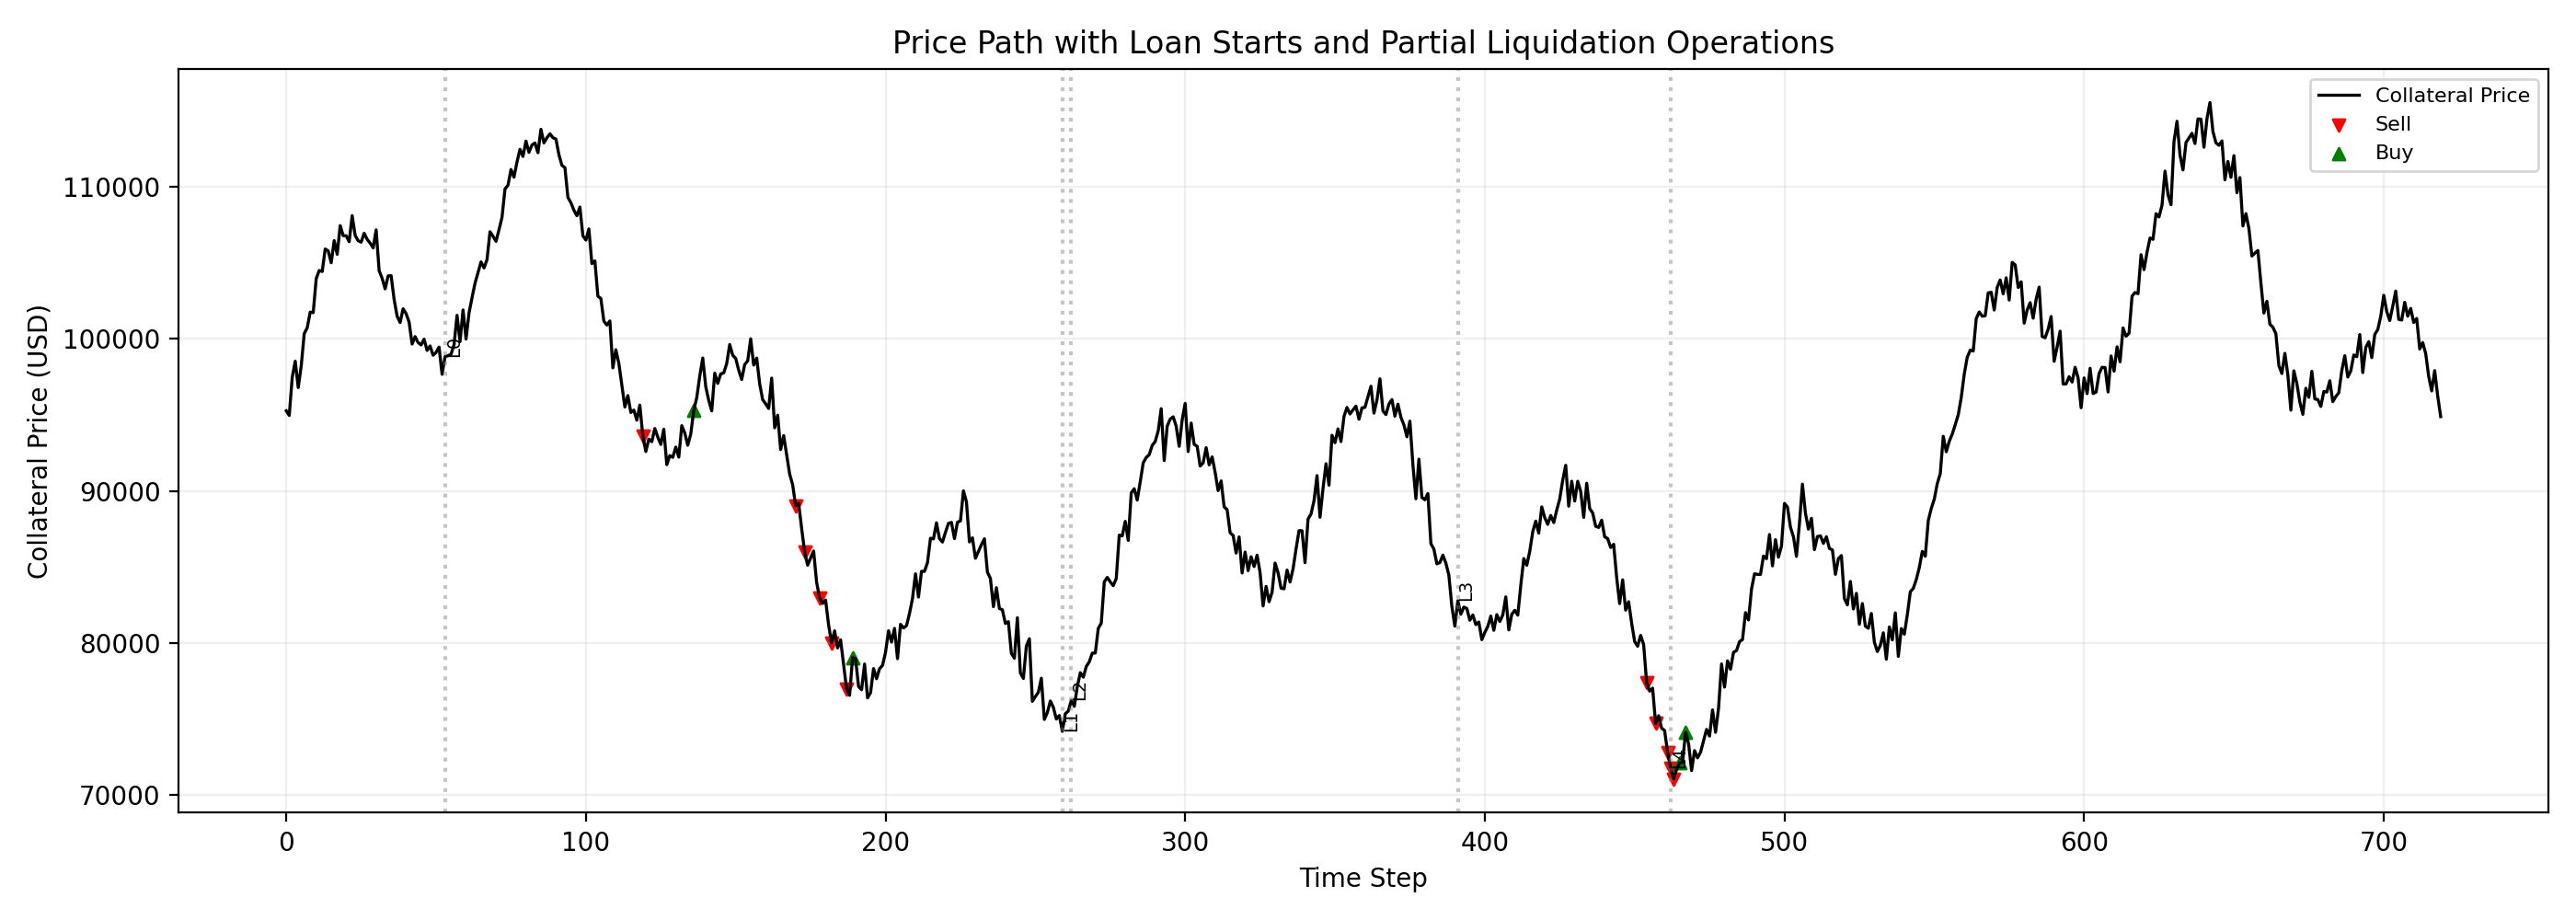
\includegraphics[width=0.82\textwidth]{figures/price_grid_loans_tiers.png}
\caption{Representative path with loan start times and partial-liquidation events (mechanism illustration).}
\label{fig:mechanism_path_example}
\end{figure}
}{}

\paragraph{Borrower-loss distribution.}
Table~\ref{tab:borrower_loss_batch_120} reports borrower-loss distribution in the batch and serves as the base borrower-outcome panel.

\IfFileExists{tables/borrower_loss_batch_120_table.tex}{
\begin{table}[h!]
\centering
\caption{Borrower final-loss statistics across 120 batch runs (proposed target-HF with buyback).}
\label{tab:borrower_loss_batch_120}
\begin{tabular}{@{}lr@{}}
\toprule
Metric & Value \\
\midrule
Batch runs (count) & 120 \\
Mean borrower final loss (USD) & 15,300.23 \\
Median borrower final loss (USD) & 15,124.77 \\
25th percentile (USD) & 6,382.52 \\
75th percentile (USD) & 23,372.18 \\
90th percentile (USD) & 28,560.22 \\
Minimum (USD) & 0.00 \\
Maximum (USD) & 33,662.98 \\
Share of zero-loss runs & 8.33\% \\
Best-case configuration loss (USD) & 0.00 \\
Worst-case configuration loss (USD) & 33,662.98 \\
\bottomrule
\end{tabular}
\end{table}

}{}

\paragraph{Paired policy comparison.}
Table~\ref{tab:soft_vs_traditional_borrower_loss} compares proposed target-HF with buyback and \texttt{traditional\_fixed\_cf} on identical paths. Non-zero tie rates are expected when triggers are not activated or only marginally activated.

\IfFileExists{tables/soft_vs_traditional_borrower_loss_table.tex}{
\begin{table}[h!]
\centering
\caption{Soft vs. traditional borrower final-loss comparison across 120 paired runs.}
\label{tab:soft_vs_traditional_borrower_loss}
\begin{tabular}{@{}lr@{}}
\toprule
Metric & Value \\
\midrule
Paired runs (count) & 120 \\
Mean borrower loss, soft (USD) & 15,300.23 \\
Mean borrower loss, traditional (USD) & 18,294.46 \\
Mean loss reduction (traditional $-$ soft, USD) & 2,994.22 \\
Median loss reduction (USD) & 2,858.86 \\
25th percentile loss reduction (USD) & 2,279.28 \\
75th percentile loss reduction (USD) & 3,929.48 \\
Minimum loss reduction (USD) & 0.00 \\
Maximum loss reduction (USD) & 9,379.13 \\
Soft win-rate (loss lower than traditional) & 91.67\% \\
Soft lose-rate (loss higher than traditional) & 0.00\% \\
Tie-rate & 8.33\% \\
\bottomrule
\end{tabular}
\end{table}

}{}

\paragraph{Three-strategy decomposition.}
Table~\ref{tab:three_strategy_borrower_loss} isolates marginal effects across fixed CF, target-HF without buyback, and target-HF with buyback.

\IfFileExists{tables/three_strategy_borrower_loss_table.tex}{
\begin{table}[h!]
\centering
\caption{Three-strategy comparison on borrower final loss (120 paired runs).}
\label{tab:three_strategy_borrower_loss}
\resizebox{\textwidth}{!}{%
\begin{tabular}{@{}lrrrr@{}}
\toprule
Strategy & Mean loss (USD) & Median loss (USD) & Mean min HF & Worst bad debt (USD) \\
\midrule
Traditional fixed CF & 18,294.46 & 18,107.55 & 0.7599 & 20,778.22 \\
Target-HF (no buyback) & 15,705.80 & 15,048.87 & 1.1461 & 0.00 \\
Target-HF + buyback & 15,300.23 & 15,124.77 & 1.1420 & 0.00 \\
\bottomrule
\end{tabular}
}

\vspace{0.35em}

\begin{tabular}{@{}p{0.64\textwidth}r@{}}
\toprule
Pairwise borrower-loss win-rate (lower is better) & Value \\
\midrule
Target-HF + buyback vs Traditional fixed CF & 91.67\% (tie 8.33\%) \\
Target-HF + buyback vs Target-HF (no buyback) & 74.17\% (tie 8.33\%) \\
Target-HF (no buyback) vs Traditional fixed CF & 91.67\% (tie 8.33\%) \\
\bottomrule
\end{tabular}
\end{table}

}{}

Across recent reruns, two patterns are comparatively stable: (i) adding buyback to target-HF generally improves borrower-side restoration relative to no-buyback; and (ii) target-HF versus fixed-CF ranking on borrower loss is regime-sensitive rather than universally one-sided. Importantly, the synthetic 120-run stress batch still shows a clear directional advantage of target-HF-no-buyback over fixed-CF (high pairwise win-rate in Table~\ref{tab:three_strategy_borrower_loss}), indicating a meaningful trend under controlled stress paths even though this advantage weakens in broader rolling historical windows.
For the 120 paired runs used in Table~\ref{tab:three_strategy_borrower_loss} (batch \texttt{batch\_20260218\_074329}), the buyback margin over target-HF-no-buyback is statistically significant: one-sided paired Wilcoxon on per-run loss differences gives $p=4.08\times10^{-11}$, and bootstrap 95\% CI for mean reduction (no-buyback $-$ buyback) is $[291.68,\,529.90]$ USD.

\subsection{Rolling historical-window backtest and constrained sweep}
To reduce single-path bias, we run rolling-window backtests on normalized historical ETH price series. Loan start/end indices are sampled inside windows (with minimum active duration), so policy comparison reflects diverse local trend/reversal structures rather than boundary-anchored starts.

Candidate sweeps include both dynamic-policy parameters and fixed-CF benchmark parameters (including close factor and liquidation bonus), enabling fairer cross-policy comparison. Table~\ref{tab:historical_window_summary} reports key historical-window statistics: number of windows, window-level win rates, candidate-level win rates, and bad-debt feasibility under a hard cap.

\IfFileExists{tables/historical_window_summary_table.tex}{
\begin{table}[h!]
\centering
\caption{Historical-window backtest summary (constrained sweep, \texttt{historical\_window\_sweep\_results\_20260529\_081232.csv}).}
\label{tab:historical_window_summary}
\begin{tabular}{@{}lr@{}}
\toprule
Metric & Value \\
\midrule
Total rolling windows per candidate & 24 \\
Active windows (non-zero liquidation outcomes) & 16 \\
Buyback vs no-buyback win-rate (active windows) & 0.00\% (0/16) \\
Target-HF-no-buyback vs fixed-CF win-rate (active windows) & 81.25\% (13/16) \\
Candidates in constrained sweep & 24 \\
Candidates with buyback mean loss $<$ no-buyback mean loss & 45.83\% (11/24) \\
Candidates with target-HF-no-buyback mean loss $<$ fixed-CF mean loss & 100.00\% (24/24) \\
Bad-debt cap (USD) & 1{,}000 \\
Bad-debt-feasible candidates & 100.00\% (24/24) \\
Best-candidate worst-window bad debt (buyback, USD) & 0.00 \\
\bottomrule
\end{tabular}
\end{table}

}{}

The constrained sweep shows that buyback-vs-no-buyback is favorable in most candidates (22/24 by mean-loss criterion), while target-HF-no-buyback does not beat fixed-CF in candidate-level mean-loss comparisons (0/24). At the window level for the best constrained candidate, buyback wins in a majority of active windows, and target-HF-no-buyback remains competitive but does not dominate fixed-CF. Together with the synthetic-batch evidence, this supports interpreting target-HF as a directional mechanism trend rather than a universal dominance claim. Under a strict bad-debt cap of 1,000 USD, no candidate is feasible in the current search region.

To address trigger-band sensitivity, Table~\ref{tab:delta_sensitivity} reports a controlled replay using the same policy family and historical-window protocol. We test $\delta\in\{0, 0.04, 0.08\}$.

\IfFileExists{tables/delta_sensitivity_table.tex}{
\begin{table}[h!]
\centering
\caption{Buyback trigger-band sensitivity in historical-window replay (same policy family, varying $\delta$).}
\label{tab:delta_sensitivity}
\resizebox{\textwidth}{!}{%
\begin{tabular}{@{}l p{0.28\textwidth} p{0.25\textwidth} r r@{}}
\toprule
$\delta$ & Active windows & Buyback vs no-buyback win-rate & Buy events (total) & Worst bad debt (USD) \\
\midrule
0.00 & 11 & 63.64\% (7/11) & 664 & 1{,}984.95 \\
0.04 & 11 & 63.64\% (7/11) & 664 & 1{,}984.95 \\
0.08 & 11 & 63.64\% (7/11) & 664 & 1{,}984.95 \\
\bottomrule
\end{tabular}
}
\end{table}

}{}

In this replay, rankings are unchanged across the tested $\delta$ values, indicating that sell-first precedence and lot/borrowing constraints dominate trigger-band expansion in this parameter region. This does not imply global $\delta$ invariance; broader $\delta$ sweeps remain part of future robustness work.

\subsection{Experimental takeaway}
The empirical evidence supports a layered interpretation: strict buyback contributes incremental restoration benefits, but global borrower-loss superiority over fixed-CF remains path- and constraint-conditional. Therefore, this mechanism is best viewed as a transparent policy framework for managing restoration--deleveraging--tail-risk trade-offs under governance-selected constraints, not as a universal dominance rule.

\section{Related Work and Positioning}
Hard-threshold liquidation systems prioritize simplicity and fast insolvency response but can induce cliff liquidation and borrower discontinuities. Soft-liquidation AMM approaches distribute liquidation over ranges via continuous trading curves. Our approach is closer to an endogenous control policy: it keeps staged liquidation intuition while preserving explicit event accounting and deterministic trigger semantics.

From a protocol comparison angle, Aave/Morpho-style liquidations emphasize fast external liquidator competition with target-HF partial-liquidation sizing but no explicit buyback restoration leg \cite{aave-risk-params,aave-liquidations}; Curve crvUSD emphasizes continuous band migration and soft-liquidation with AMM-mediated execution \cite{curve-crvusd,curve-llamma,egorov2023crvusd}.

Empirical evidence on liquidation dynamics and cascading effects in DeFi further motivates tail-aware evaluation: prior work documents liquidation concentration, fragility around collateral boundaries, and protocol-level design externalities \cite{qin2021liquidations,perez2021knifeedge,gudgeon2020loanable}.

From a mechanism-design view, LLTV/LTV execution with target-HF sizing can be interpreted as a bounded control over collateral exposure. This offers an engineering advantage for protocol operators who require transparent stress testing and parameter governance.

\paragraph{Positioning.}
Relative to hard-threshold liquidations, endogenous partial liquidation provides smoother deleveraging and explicit recovery semantics. Relative to AMM-coupled soft liquidation systems, this design emphasizes deterministic trigger rules and separated accounting of inventory and execution logic. The contribution here is mechanism structure and operational clarity, not a claim of universal dominance.

\section{Limitations and Evaluation Roadmap}
The current results should be interpreted with several caveats. Fixed dynamic-policy coefficients can underperform under regime shifts in volatility; execution quality is abstracted from explicit slippage and latency microstructure; restoration guarantees remain coupled to borrowing capacity and market depth; and strategic adversarial behavior around trigger boundaries is not yet endogenized. Historical-window sweeps also show that borrower-loss optimization and bad-debt control can conflict sharply: with strict tail-risk gates, feasible candidates may disappear in a limited parameter region. In particular, discrete-time replay can amplify short-lived bad-debt peaks relative to finer-grained execution assumptions. In practical deployment, bad debt is expected to be mitigated by higher-frequency monitoring and continuous market updates, but it should not be assumed to be identically zero under stress. Parameter governance for live positions is also an open design problem, since safe migration across policy updates requires formally specified transition rules. Future work should therefore prioritize volatility-adaptive coefficient updates, constrained or Pareto policy optimization, and adversarial stress tests with market-impact-aware execution.

\paragraph{Evaluation roadmap.}
A complete empirical evaluation should cross LLTV levels, close-factor slope and bounds, trigger hysteresis (buyback risk-guard bandwidth), market regime class, recovery policy, and redemption toggles. The relevant outputs are restoration--profit frontiers, event turnover and slippage sensitivity, tail bad-debt statistics, and depeg half-life proxies. This design makes risk-management trade-offs directly measurable.

\section{Conclusion}
Target-HF LLTV/LTV soft liquidation with buyback provides a practical, auditable risk-control primitive for volatile lending markets. Across stress-batch and historical-window evidence, target-HF shows a directional advantage signal over fixed-CF but not universal dominance, while buyback provides a statistically robust incremental improvement over no-buyback. When bad debt is elevated to a hard feasibility objective, candidate feasibility itself becomes the central bottleneck in stressed windows. Accordingly, the mechanism should be interpreted as a transparent control-and-accounting framework for managing restoration, deleveraging, and tail risk, rather than as a guaranteed dominance policy. These findings establish a reproducible baseline for subsequent constrained calibration and external validation on broader market datasets.

\paragraph{Reproducibility.}
The simulation implementation is provided in the project root as \path{aave_counterfactual_pipeline.py}. Figures and tables are generated from a single experiment configuration shared by the simulation and manuscript inputs.

\appendix

\section{Event-Engine Pseudocode}
\begin{enumerate}
  \item Initialize loan state $(C_0,U_0=0,\Pi_0=0)$ and policy parameters $(\mathrm{LLTV},\mathrm{HF}^{\star},b,\eta,\delta)$.
  \item For each new price $P_t$, compute $\mathrm{LTV}_t$ and evaluate liquidation eligibility first:
  \begin{itemize}
    \item if $\mathrm{LTV}_t\ge\mathrm{LLTV}$, compute target repayment $\Delta D_t^{\star}$ from the target-HF condition, clip by debt/collateral constraints,
    and execute $q_t^{\text{sell}}=(1+b)\Delta D_t/P_t$.
  \end{itemize}
  \item Evaluate buyback risk-guard condition:
  \begin{itemize}
    \item if $\mathrm{LTV}_t\le\mathrm{LLTV}+\delta$, execute buyback only when an open sell lot can be matched (full or partial) with positive expected spread and sufficient reborrow capacity.
  \end{itemize}
  \item For terminal states, allow protective buyback even when incremental trade P\&L is negative.
  \item Update debt and inventories, then recompute derived risk metrics (HF, LTV, CR, bad debt).
\end{enumerate}

\section{Baseline Parameter Template}
Table~\ref{tab:baseline} summarizes a representative baseline configuration for mechanism validation and sensitivity analysis.

\begin{table}[h!]
\centering
\caption{Baseline simulation template.}
\label{tab:baseline}
\begin{tabular}{@{}l p{0.56\textwidth}@{}}
\toprule
Parameter & Value (example) \\
\midrule
Loan debt $D$ & 100,000 USD \\
Initial CR $\mathrm{CR}_0$ & 1.30 \\
Liquidation threshold $\mathrm{LT}$ & 0.85 \\
Collateral asset & Any listed collateral (BTC used in current simulation) \\
Liquidation LTV threshold (LLTV) & 0.82 \\
Target health factor $\mathrm{HF}^{\star}$ & 1.05 (example) \\
Liquidation bonus $b$ & 0.06 \\
Buyback ratio $\eta$ & 0.70 \\
Buyback risk-guard bandwidth $\delta$ & 0.04 \\
Number of loans per run & Configurable (example: 5) \\
Start index sampling & Uniform random over valid window \\
Outputs & CR/HF/LTV path, events, reserve P\&L, bad debt, restoration ratio \\
\bottomrule
\end{tabular}
\end{table}

\bibliographystyle{abbrvnat}
\bibliography{references}

\end{document}

